\documentclass[10pt,letterpaper]{article}
\usepackage[top=0.50in,bottom=0.52in,left=0.62in,right=0.62in,headheight=14pt,headsep=5pt,footskip=15pt]{geometry}
\usepackage{fontspec}
\setmainfont{Noto Serif}
\setsansfont{Noto Sans}
\usepackage[spanish,es-noshorthands]{babel}
\usepackage{microtype,ragged2e,setspace}
\usepackage{graphicx}
\graphicspath{{figures/}}
\usepackage{booktabs,tabularx,array,multirow,longtable}
\usepackage[table]{xcolor}
\usepackage{fancyhdr,hyperref,enumitem,multicol}

\definecolor{autumn}{HTML}{E36A2E}
\definecolor{spicy}{HTML}{C8572A}
\definecolor{onyx}{HTML}{0C0C0C}
\colorlet{orange}{autumn}
\colorlet{ink}{onyx}
\colorlet{muted}{onyx!58!white}
\colorlet{rule}{onyx!18!white}
\definecolor{soft}{HTML}{F5F7FA}
\definecolor{softblue}{HTML}{EAF2FD}
\definecolor{softgreen}{HTML}{EAF7EF}
\definecolor{softwarm}{HTML}{FDEFE8}

\hypersetup{colorlinks=true,urlcolor=spicy,linkcolor=spicy,pdftitle={Marco teorico y estado del arte para el TFM MROB},pdfauthor={Jorge Luis Mayorga Taborda}}
\pagestyle{fancy}\fancyhf{}
\fancyhead[L]{\sffamily\fontsize{7.3}{8}\selectfont Jorge Luis Mayorga Taborda}
\fancyhead[R]{\sffamily\fontsize{7.3}{8}\selectfont TFM MROB · Marco teórico y estado del arte}
\fancyfoot[C]{\sffamily\fontsize{8.2}{8.7}\selectfont\thepage}
\renewcommand{\headrulewidth}{0.25pt}
\setlength{\parindent}{0pt}\setlength{\parskip}{2.2pt}
\setstretch{1.05}\color{ink}\emergencystretch=1.4em
\setlist[enumerate]{leftmargin=3.7mm,itemsep=0pt,topsep=0pt,parsep=0pt,partopsep=0pt}

\newcommand{\sect}[1]{\par\vspace{0pt}{\sffamily\fontsize{14.5}{15.5}\selectfont\bfseries\color{orange}#1\par}\vspace{1.2pt}\textcolor{rule}{\rule{\linewidth}{0.35pt}}\vspace{3pt}}
\newcommand{\subh}[1]{\par\vspace{2.2pt}{\sffamily\fontsize{9.3}{10.2}\selectfont\bfseries\color{orange}#1\par}\vspace{.5pt}}
\newcommand{\figcap}[2]{\par\vspace{1.0pt}{\setstretch{1}\fontsize{8.1}{8.9}\selectfont\textbf{#1.}~\textit{#2}\par}\vspace{1.0pt}}
\newcommand{\sourcecap}[1]{\par{\setstretch{1}\fontsize{7.0}{7.7}\selectfont\itshape\centering Fuente: #1\par}}

\begin{document}
\setcounter{page}{4}

% ================= REPLACEMENT PAGE 4 =================
\fontsize{8.25}{8.95}\selectfont
A partir de esa codificación por etapas, el análisis temporal amplía la comparación del núcleo curado sin mezclar volumen con composición. Cada documento distribuye un peso total de uno entre siete familias y las cuotas se calculan dentro de cuatro periodos. Las curvas describen el corpus adquirido; no estiman la prevalencia del campo ni convierten una mención de título o resumen en evidencia de implementación.
\normalsize
\begin{center}
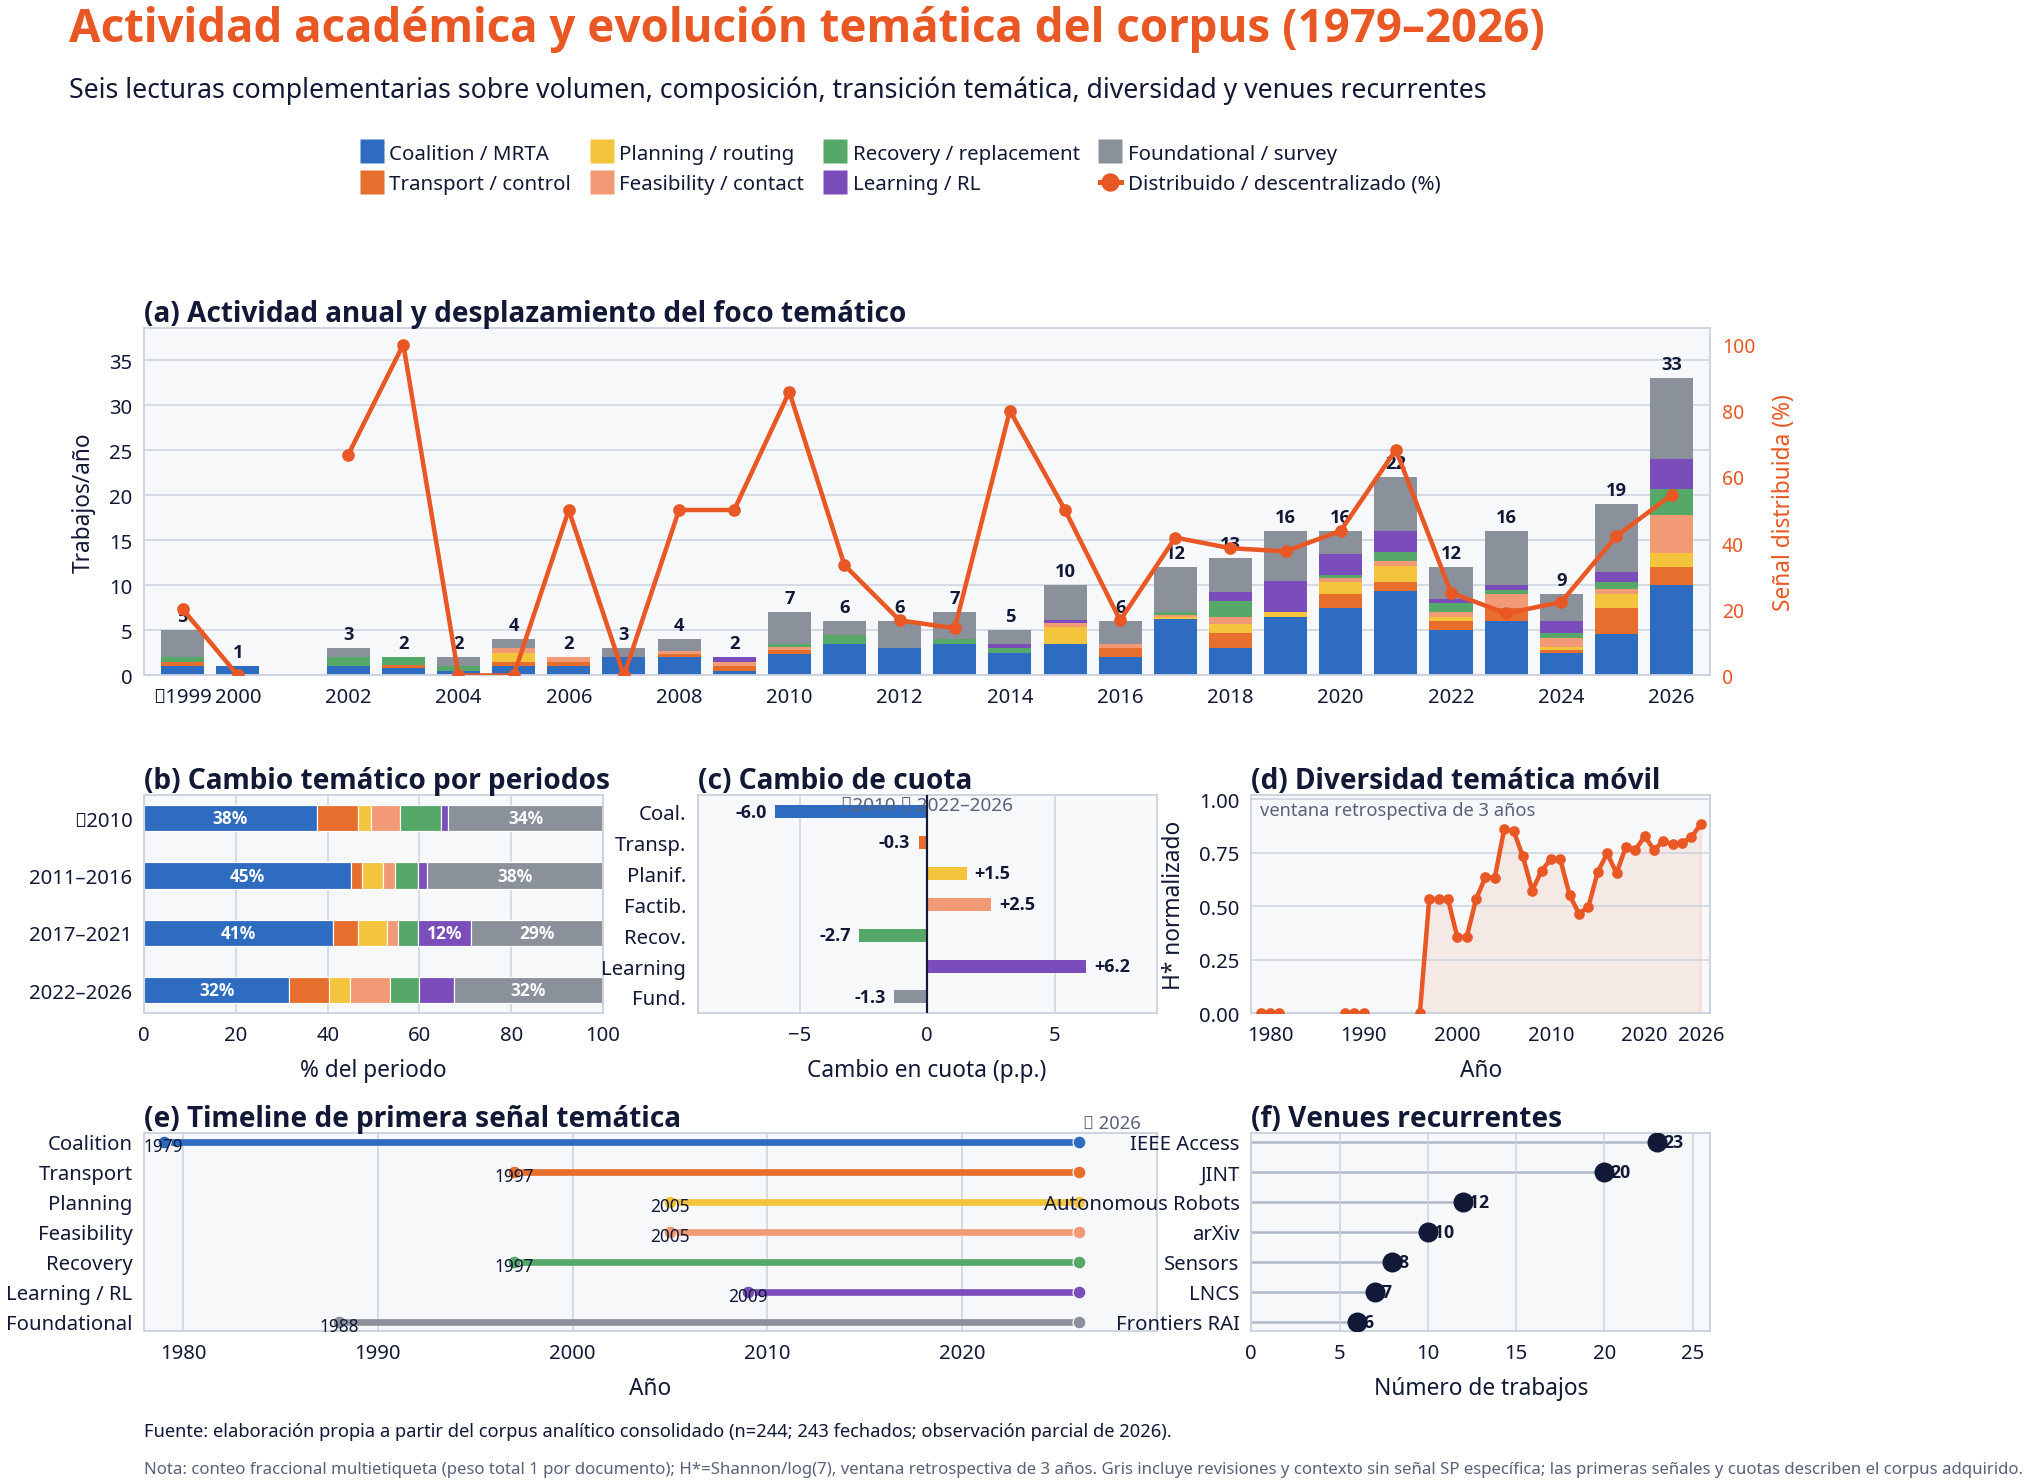
\includegraphics[width=0.985\linewidth]{fig04_academic_trends_full_corpus.pdf}
\end{center}
\figcap{Figura 4}{Actividad académica y evolución temática del corpus analítico completo (1979--2026). El panel (a) combina volumen, composición fraccional y señal distribuida; (b)--(f) muestran cuotas por periodo, cambio de cuota, diversidad móvil, primera señal observada y venues recurrentes.}
\sourcecap{corpus analítico consolidado, $n=244$; 243 documentos fechados y observación parcial de 2026. Las señales de título y resumen describen el corpus adquirido, no prevalencia poblacional ni implementación.}

\fontsize{8.35}{9.10}\selectfont
La serie no muestra el reemplazo de una familia metodológica por otra. Subastas, consenso, formación y optimización permanecen, mientras aprendizaje, seguridad y factibilidad se incorporan a combinaciones más diversas. Entre el primer periodo y 2022--2026, aprendizaje aumenta 6,2 puntos porcentuales, factibilidad 2,5 y planificación 1,5; coalición/MRTA cede 6,0 puntos y recuperación 2,7, mientras transporte apenas cambia. El desplazamiento es composicional: se amplía la combinación de métodos, pero no desaparecen las familias que originaron el campo.

La diversidad móvil reciente se aproxima a 0,89 y la señal distribuida fluctúa de un año a otro. Por ello, ninguna de las dos curvas acredita por sí sola una transición hacia arquitecturas completamente distribuidas. La dispersión entre 117 venues impone la misma cautela: la evolución no puede reconstruirse desde una sola revista, comunidad de autores o etiqueta temática.

Los cambios de cuota no revelan por sí solos dónde se concentra la evidencia. La Figura 5 separa las familias metodológicas dentro de cada periodo y la Figura 6 localiza la validación en SP1, SP2 y SP3. El interés ya no está en cuántos documentos se publican, sino en qué interfaces llegan a cubrir y con qué clase de contraste.
\normalsize

\newpage
\setcounter{page}{7}
% ================= NEW PAGE 7 =================
\normalsize
\fontsize{8.15}{8.85}\selectfont
La discontinuidad técnica también aparece en la organización del corpus. La red de coautoría conserva firmas con al menos dos documentos y componentes de tres o más autores. La red temática enlaza señales que coocurren en dos o más registros, ponderadas por asociación normalizada, y las agrupa mediante Louvain con semilla fija. El perfil autor--tema usa conteo fraccional. Estas redes describen colaboración y proximidad temática; no miden impacto ni calidad.
\normalsize
\begin{center}
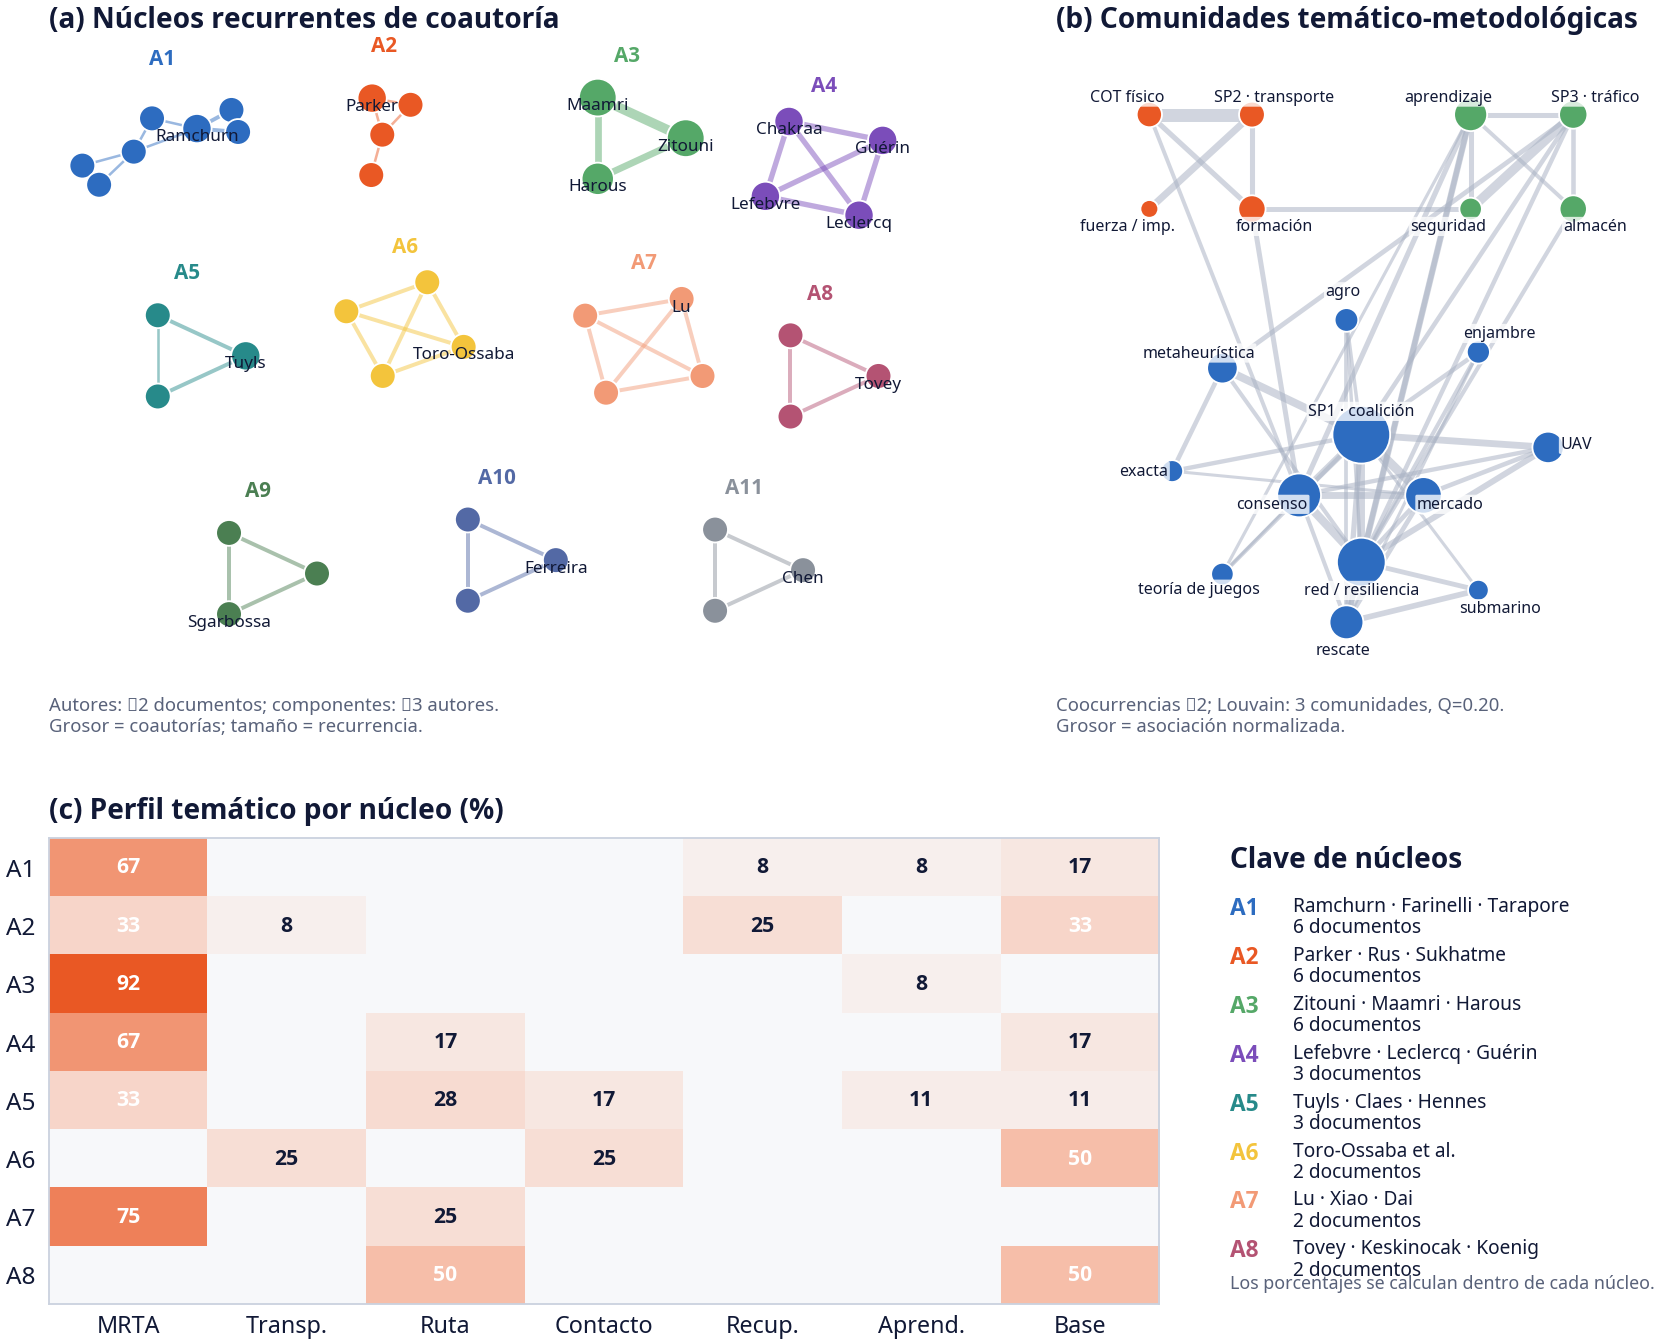
\includegraphics[width=\linewidth]{fig08_bibliometric_clusters_full_corpus.pdf}
\end{center}
\figcap{Figura 8}{Estructura bibliométrica del corpus analítico. (a) Componentes recurrentes de coautoría; (b) comunidades de coocurrencia entre temas, métodos y aplicaciones; (c) perfil temático fraccional de los ocho núcleos con mayor cobertura documental.}
\sourcecap{elaboración propia a partir de 244 registros. Los nombres corresponden a firmas exactas sin desambiguación por ORCID; los núcleos no representan rangos de impacto.}

\vspace{1.0mm}
\fontsize{7.55}{8.25}\selectfont
La estructura temática distingue tres comunidades funcionales. La primera concentra SP1, consenso, mercados y comunicación o resiliencia; la segunda reúne SP2, transporte cooperativo, formación y control de fuerza; la tercera asocia SP3 con aprendizaje, seguridad y almacenes. La modularidad baja ($Q=0{,}20$) indica que estos límites son permeables. La conexión, sin embargo, no es simétrica: SP1 coocurre diez veces con SP3 y solo dos con SP2, mientras no se observa una coocurrencia directa SP2--SP3. El cuello de botella se sitúa entre la física de la coalición cargada y la planificación del espacio que ocupa.

La red de autores aporta una lectura secundaria. Las 807 firmas contienen 72 autores recurrentes y forman 11 núcleos de al menos tres miembros. Los perfiles más estables se especializan por capa: los núcleos A1 y A3 se concentran en coalición/MRTA, A6 en transporte y factibilidad, y A8 en planificación. A2 y A5 combinan más familias, pero ningún núcleo recurrente cubre de forma clara SP1, SP2 y SP3. El resultado sugiere una producción especializada y algunos puentes parciales; no permite atribuir influencia ni explicar causalmente la brecha, pues las firmas no están desambiguadas y cada núcleo reúne entre dos y seis documentos.

La dispersión editorial refuerza la misma precaución. Los 244 documentos proceden de 117 venues; \emph{IEEE Access} aporta 23 y \emph{JINT} 20, por lo que ninguna fuente alcanza el 10\% del corpus. Las redes muestran ideas que se recombinan entre comunidades, aunque la colaboración recurrente y la evidencia técnica permanecen segmentadas. La aportación del TFM se sitúa en contratos verificables entre capas, en especial en la transferencia entre factibilidad física, tráfico y recuperación.
\normalsize

\end{document}
